\subsection{Results and Analysis} \label{Result section}
\todo{This section needs update.}
\subsubsection{Sampling Gradients results}
\begin{table}
    \centering
    \begin{tabular}{|| l l l ||}
        \hline
        \textbf{Ansatz} & \textbf{Method}                         & \textbf{Variance exponential fit} \\[0.5ex]
        \hline \hline
        Real Amplitude  & \#0: No restriction                     & -0.63                             \\
        \hline
        Real Amplitude  & \#1: Local Cost function, shallow depth & -0.06                             \\
        \hline
        Real Amplitude  & \#2: Layerwise Learning                 & -0.57                             \\
        \hline
        Customised      & \#3: Identity Blocks                    & -0.60                             \\
        \hline
    \end{tabular}
    \caption{
        The phase one of the experiments that we implemented in the Python Notebook.
        We test the same ansatzes with different methods, we record the results as the vanishing rate of gradient when the number of qubits increased.
        The differences between the \emph{fit} values are small.
        However, consider the unit measure is \emph{exponential} (i.e. $10^{-1}, 10^{-2}$) the growth or decay rates can be significant.
    }
    \label{Tab: Experiment Phase 1 Res}
\end{table}

Table \ref{Tab: Experiment Phase 1 Res} states all the combinations of ansatzes and methods.

The ansatz gradient variances decay as expected for the unrestricted setting.
The decay rate is exponentially fitted with the rate of -0.63.
The figure \ref{Plot ansatzes variance}a shows the results of the ansatz in this configuration.
The semi-log plots portray the variances of gradient from the ansatz in the unrestricted configuration.
Consider that the unit measure for variance is in \emph{exponential} form, so the linear graph is exponentially closer to zero for each qubit added to the circuit.
This result indicates that the cost function landscape becomes flatter and flatter.
Eventually, the gradient would reach a near-zero value across a large plateau, which would be inefficient for any gradient-based optimization algorithm to train the model.
We discussed this phenomenon in Section \ref{Barren Plateaus section}.


\begin{figure}
    \centering
    \begin{subfigure}[b]{.49\textwidth}
        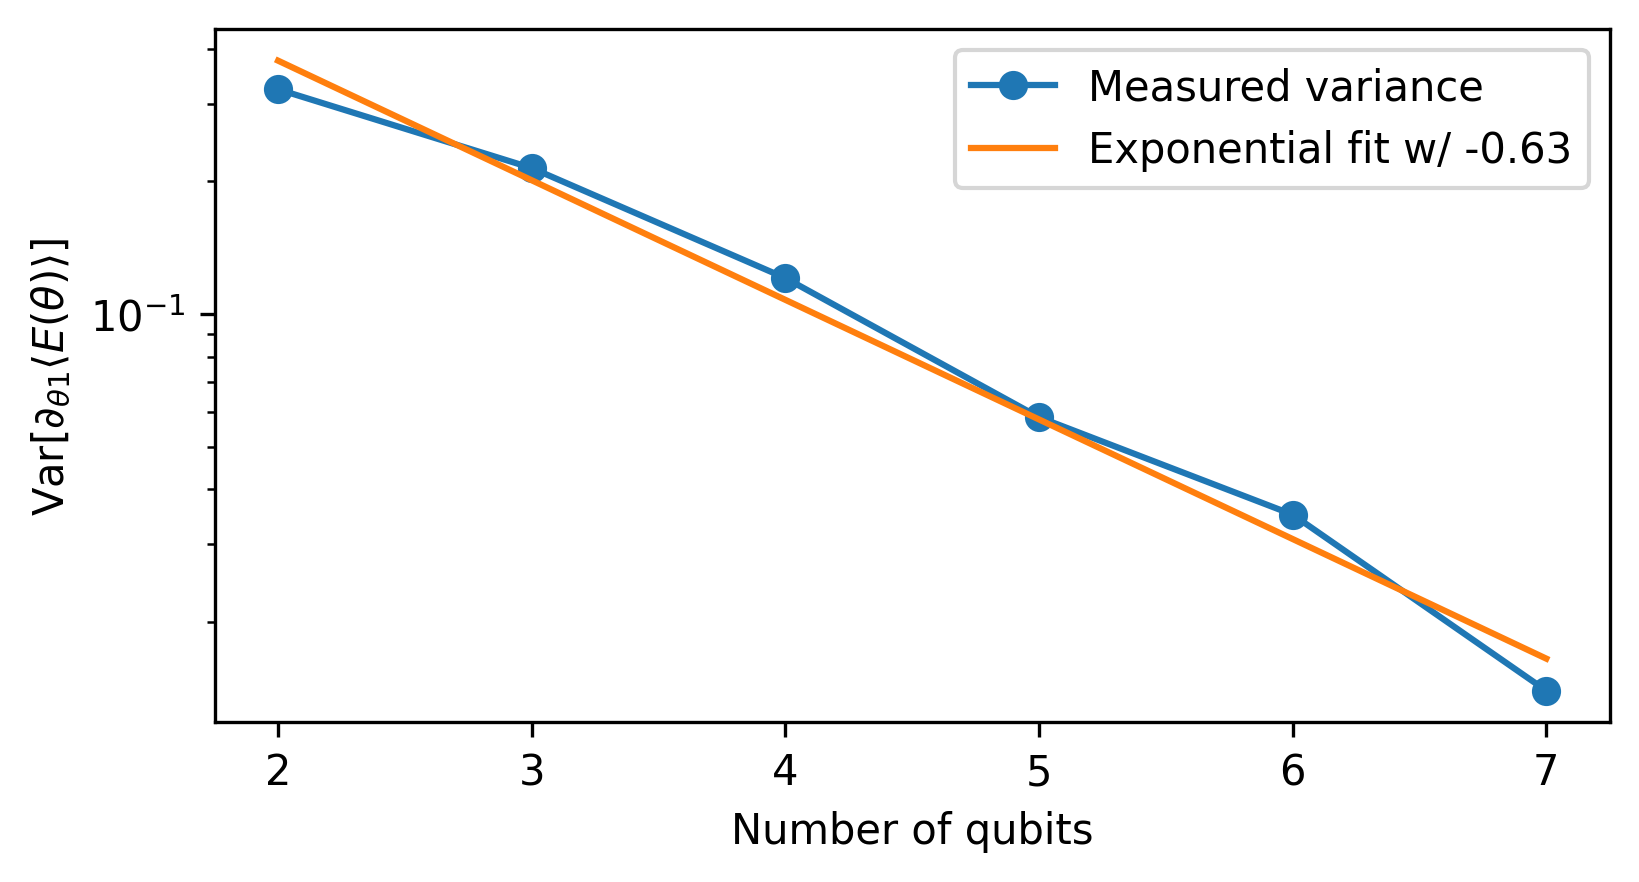
\includegraphics[width=\textwidth]{Artefact/Appendices/var0.png}
        \centerline{a) Method \#0 variances}
    \end{subfigure}
    \hfill
    \begin{subfigure}[b]{.49\textwidth}
        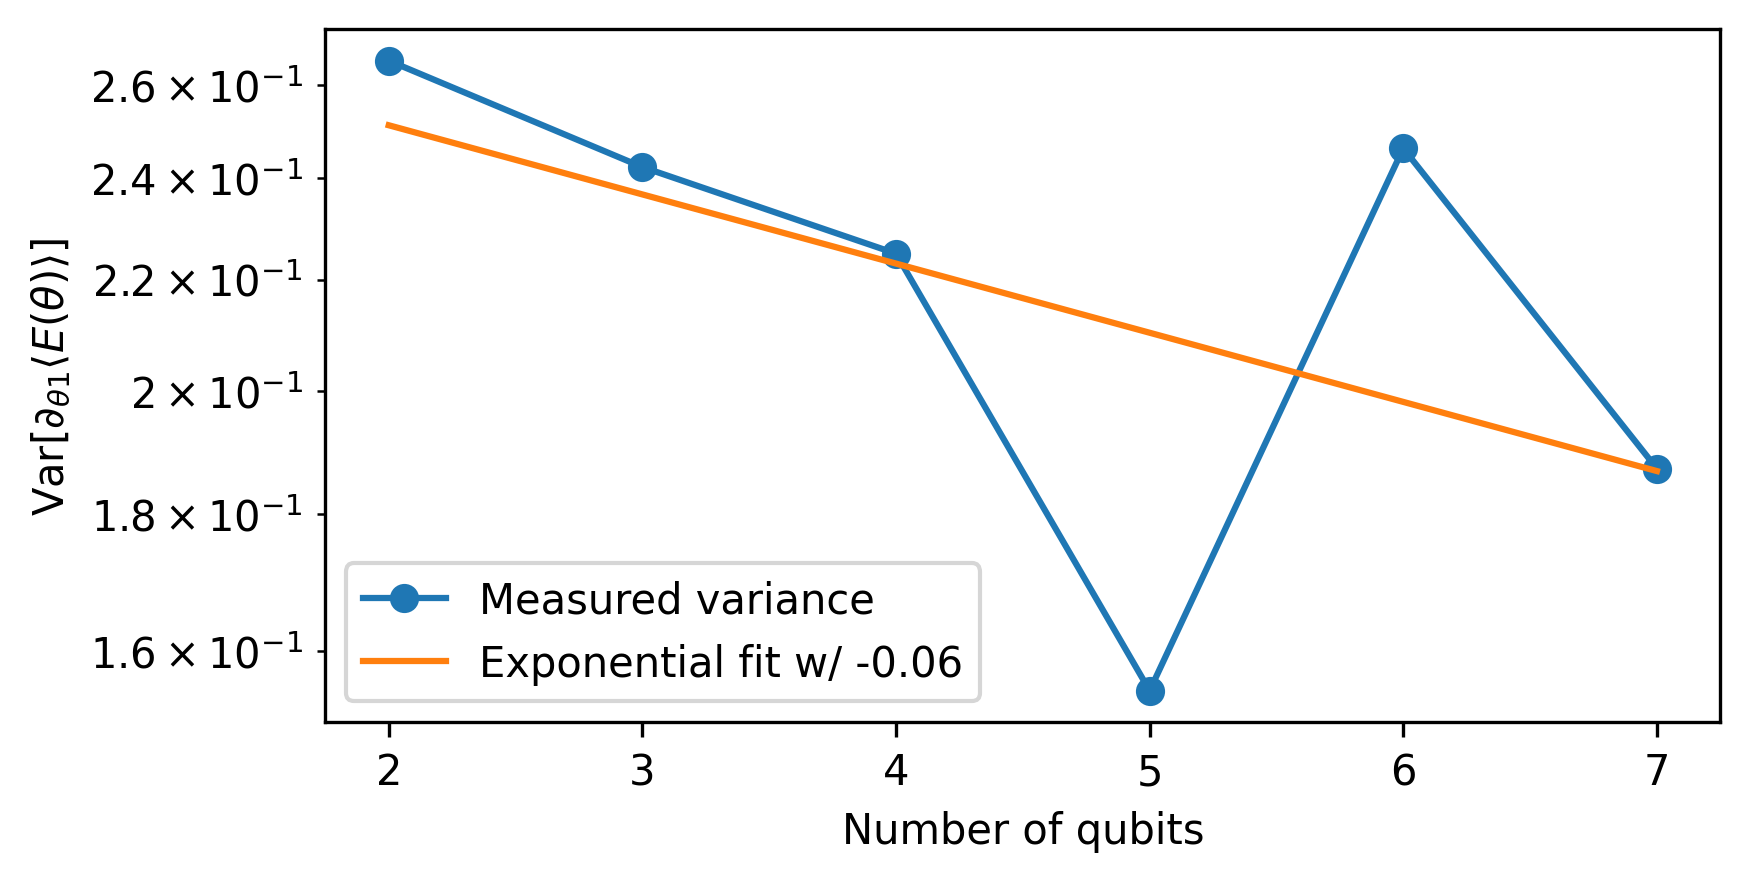
\includegraphics[width=\textwidth]{Artefact/Appendices/var1.png}
        \centerline{b) Method \#1 variances}
    \end{subfigure}

    \begin{subfigure}[b]{.49\textwidth}
        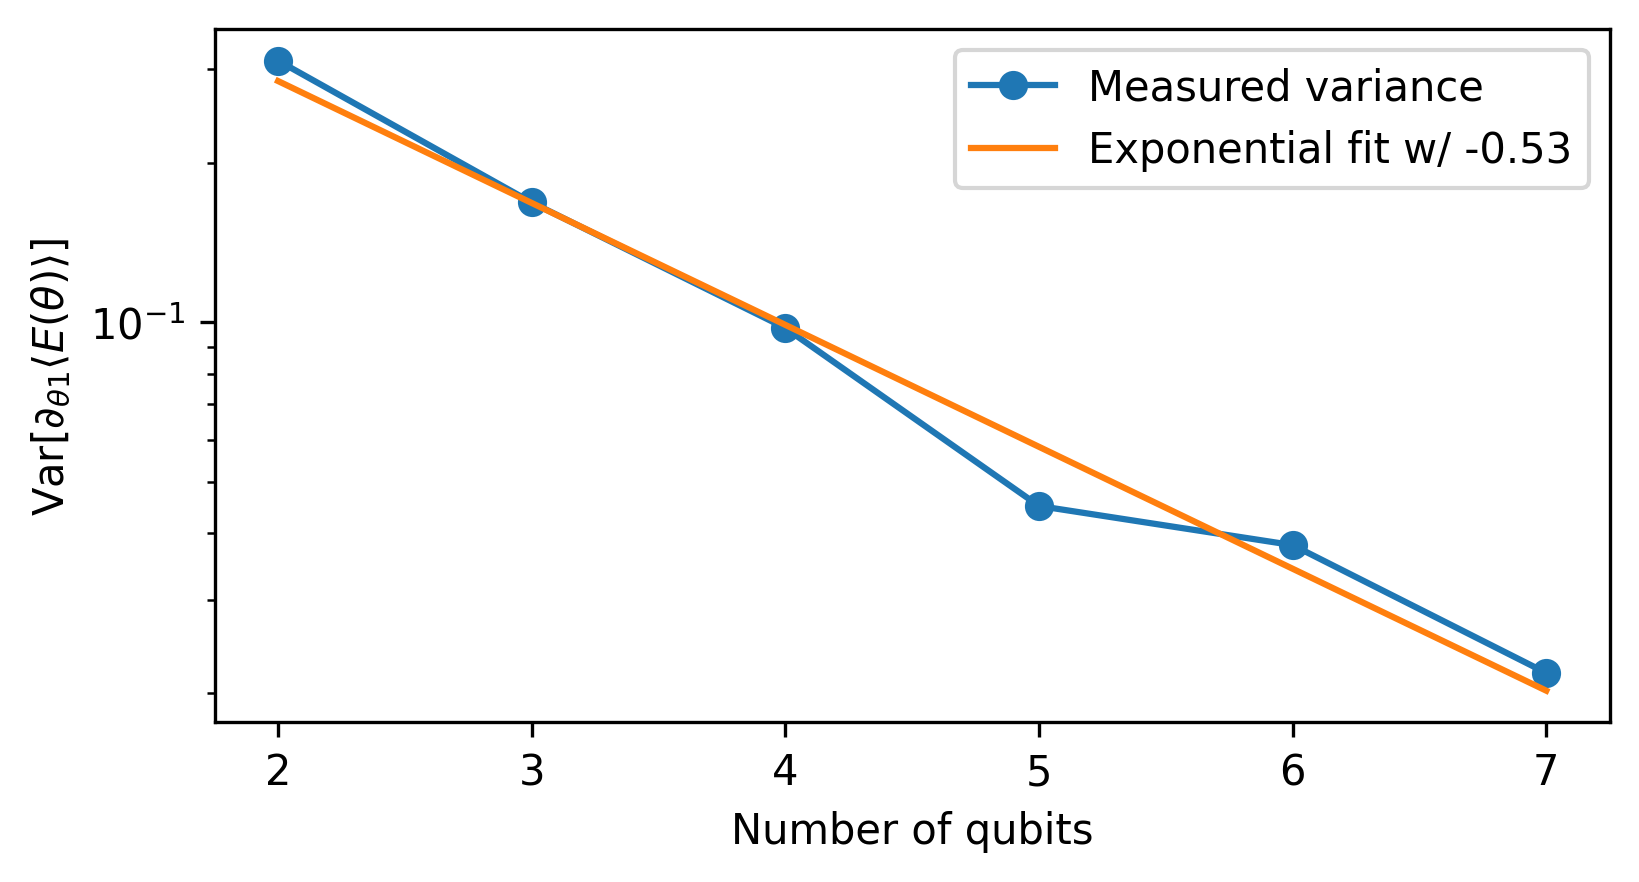
\includegraphics[width=\textwidth]{Artefact/Appendices/var2.png}
        \centerline{c) Method \#2 variances}
    \end{subfigure}
    \hfill
    \begin{subfigure}[b]{.49\textwidth}
        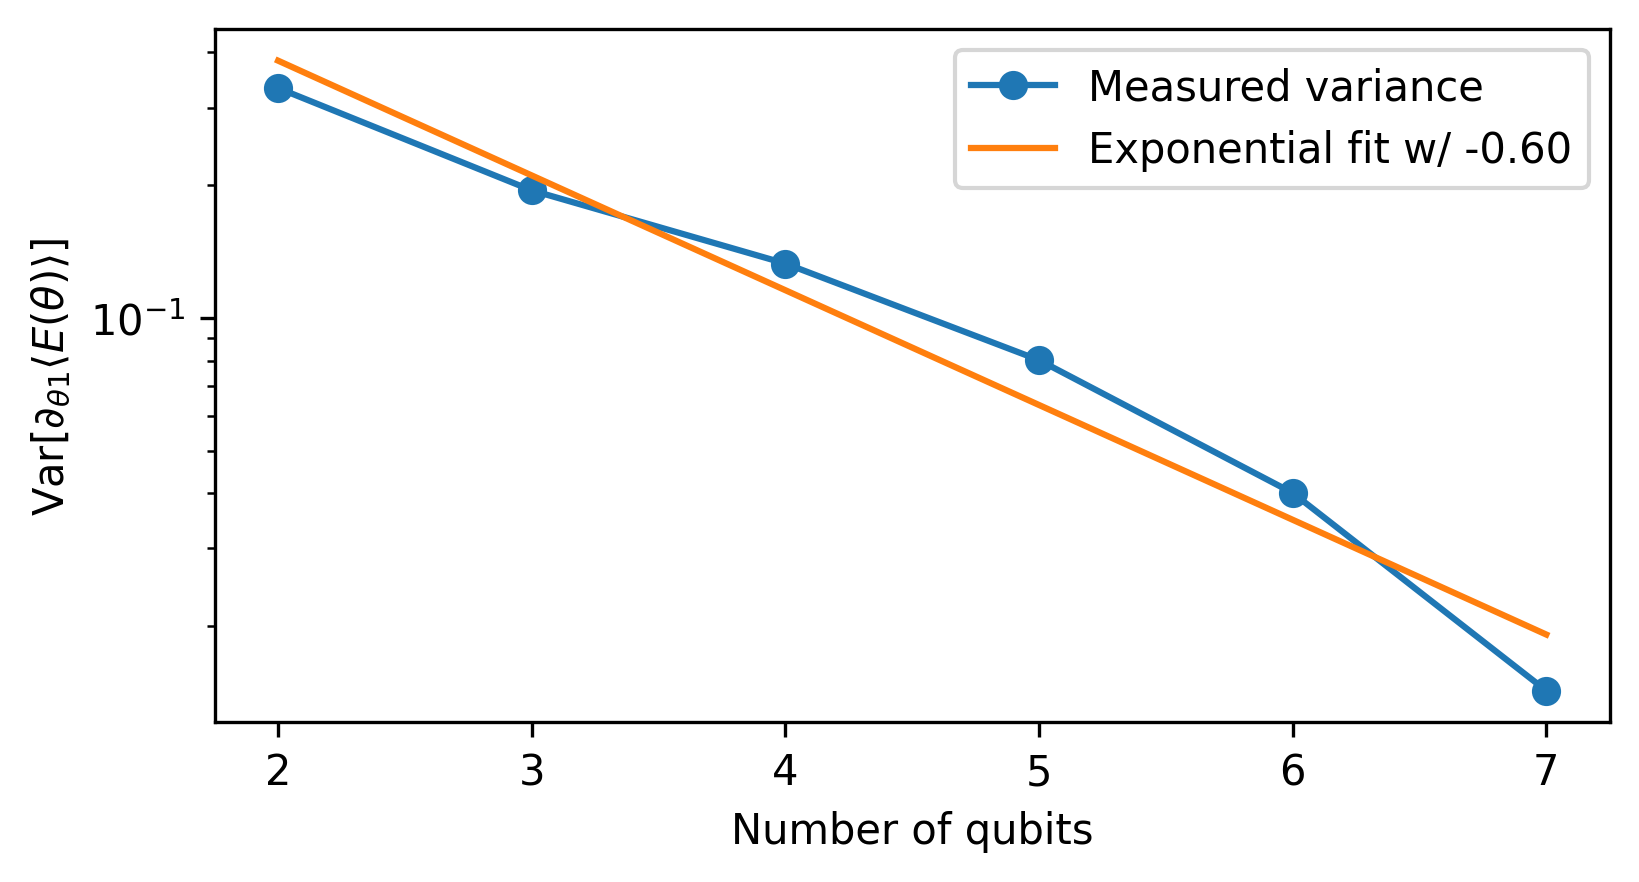
\includegraphics[width=\textwidth]{Artefact/Appendices/var3.png}
        \centerline{d) Method \#3 variances}
    \end{subfigure}

    \caption{
        The variances of gradient from differences ansatzes in the four configurations.
        For each iteration, we increase the qubit and repetition count by 1, starting from 2 to 7.
        The variances vanish exponentially to the number of qubits.
        For method \#1, we keep the repetition value fixed as 1.
    }
    \label{Plot ansatzes variance}
\end{figure}

In contrast, for the case of Local Cost Function and Shallow circuit, we observe that the variances of the ansatz' gradient did not vanish when we attempted to increase the number of qubits.
The slope of the ansat in this case decay exponentially fit with -0.06.
This implies that the cost function landscape can sustain the slope.
Figure \ref{Plot ansatzes variance}b shows the result of the experiment for local cost function and shallow circuit.
We can see that the ansatz produced an unstable graph which mean the trainability of gradient-based optimization algorithms would not be consistent.
For example, the variance value for 6 qubits is higher compared to 3, 4 or 5 qubits.

To compare the effectiveness of the different treatments, we plot the variance graph of above mention cases in Figure \ref{Fig: Plot Variances} and the Table \ref{Tab: Experiment Phase 1 Res}.
The results have shown the differences in the decay rates of different ansatzes and methods.
Overall, the ansatzes with the local cost function and restriction on circuit depth have their variance values remaining higher and being more consistent for higher qubit count.
The ansatz with this treatment, therefore would not possess a barren plateau.
On the other hand, the values for the the other cases shrink exponentially and eventually, the near-zero gradient around the initial point will expand to a large plateau.


\begin{figure}
    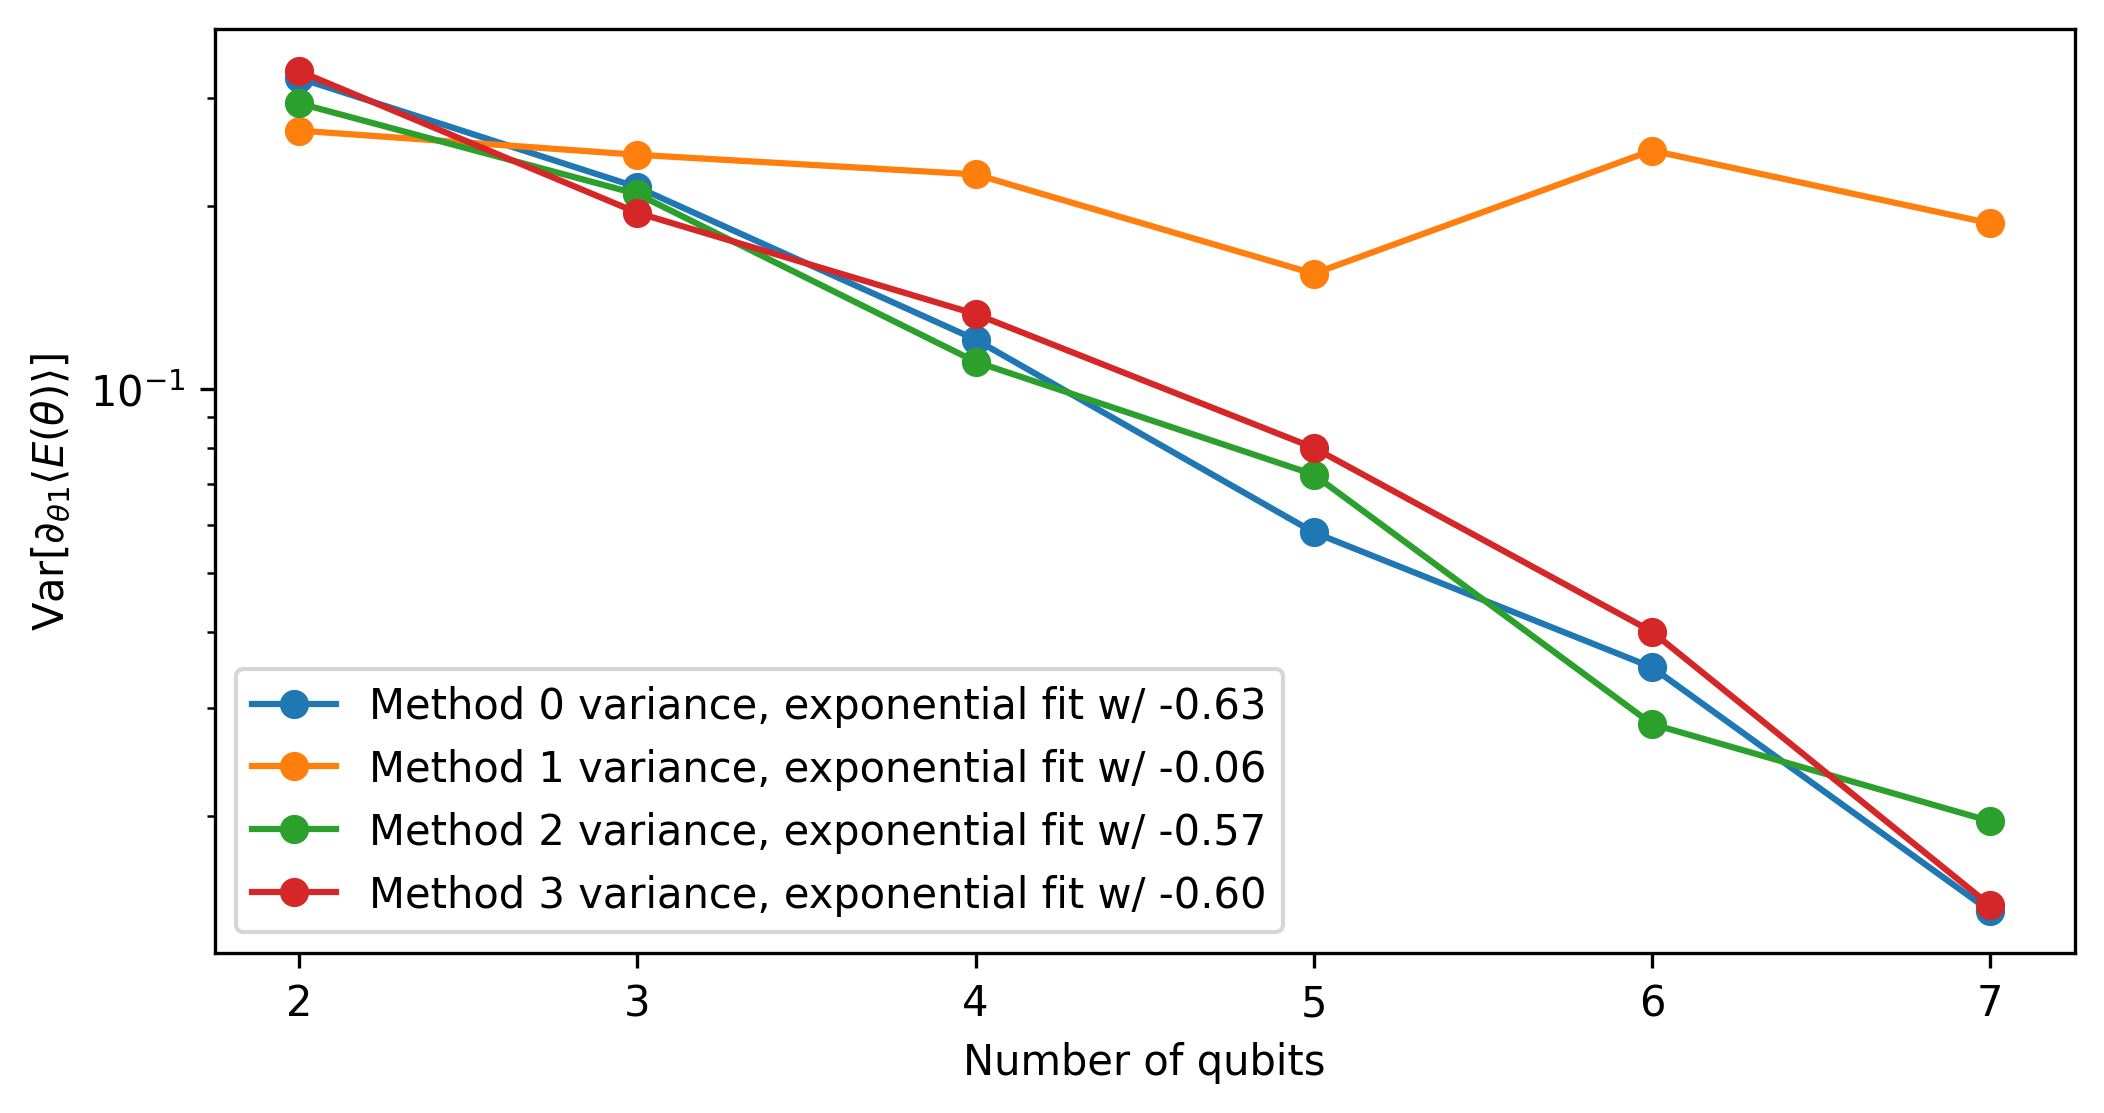
\includegraphics[width=\textwidth]{Artefact/Appendices/variances.png}
    \caption{
        Comparison of the variance values of the ansatzes with four treatments applies.
        The ansatz with local cost function and fixed depth has its variance decay at a significantly smaller rate (-0.06) compared to the rest.
    }
    \label{Fig: Plot Variances}
\end{figure}


\subsubsection{Classification Results}

\begin{table}
    \centering
    \begin{tabular}{|| l l l l l ||}
        \hline
        \textbf{Method} & \textbf{Circuit depth} & \textbf{Parameters count} & \textbf{Minimum loss} & \textbf{Score} \\
        \hline \hline
        \#0             & 15                     & 16                        & 0.57                  & 72.50\%        \\
        \#1             & 5                      & 6                         & 0.57                  & 80\%           \\
        \#2             & 15                     & 16                        & 0.39                  & 92.5\%         \\
        \#3             & 18                     & 24                        & 0.39                  & 90\%           \\
        \hline
    \end{tabular}
    \caption{
        The result as recorded from the phase two of the experiment.
        We use the ansatzes from four methods as the neural network to solve a classification problem.
    }
    \label{Tab: Experiment Phase 2 Res}
\end{table}

The method 0 and 1 loss functions both converged at value 0.57.
However, we can see that the method 1 achieved a higher accuracy in the classification test, which is 80\% compared to method 1 with 72.5\%.
However, by restricting the ansatz depth, we may have limited the model capacity and learnability of the network, this also applies to classical machine learning \cite{ianDeepLearningAdaptive2016}.
The method 1 is thus suitable if the dataset represents a simple function, as more complex function would require higher model capacity, thus higher layer count and qubit count.

The method 3 can also achieve similar loss value as method 2 (0.39) with a bit lower in accuracy.
We can see that with the optimised initial parameters, the loss function can converge faster compared to identity blocks initialisation.
However, it would take more time to obtain the optimal initial parameter due to the training process (see Section \ref{Sec: Method2}), while it is much faster to generate an parameters array for ansatz in Section \ref{Sec: Method3}.
The two methods also have their accuracy close to each other, score at 92\% for method 2 and 90\% for method 3.
Thus method 2 and 3 is thus suitable for designing ansatz of higher layer count to learn more complex functions.


To compare the effectiveness of different approaches, we plot the loss per iteration graph of above mention cases in Figure \ref{Fig: Plot Loss and Accuracy} and Table \ref{Tab: Experiment Phase 2 Res}
Overall, the methods that involve configurations on the initial parameters can achieve lower loss in training and higher score in the classification test.

\begin{figure}
    \begin{subfigure}{\textwidth}
        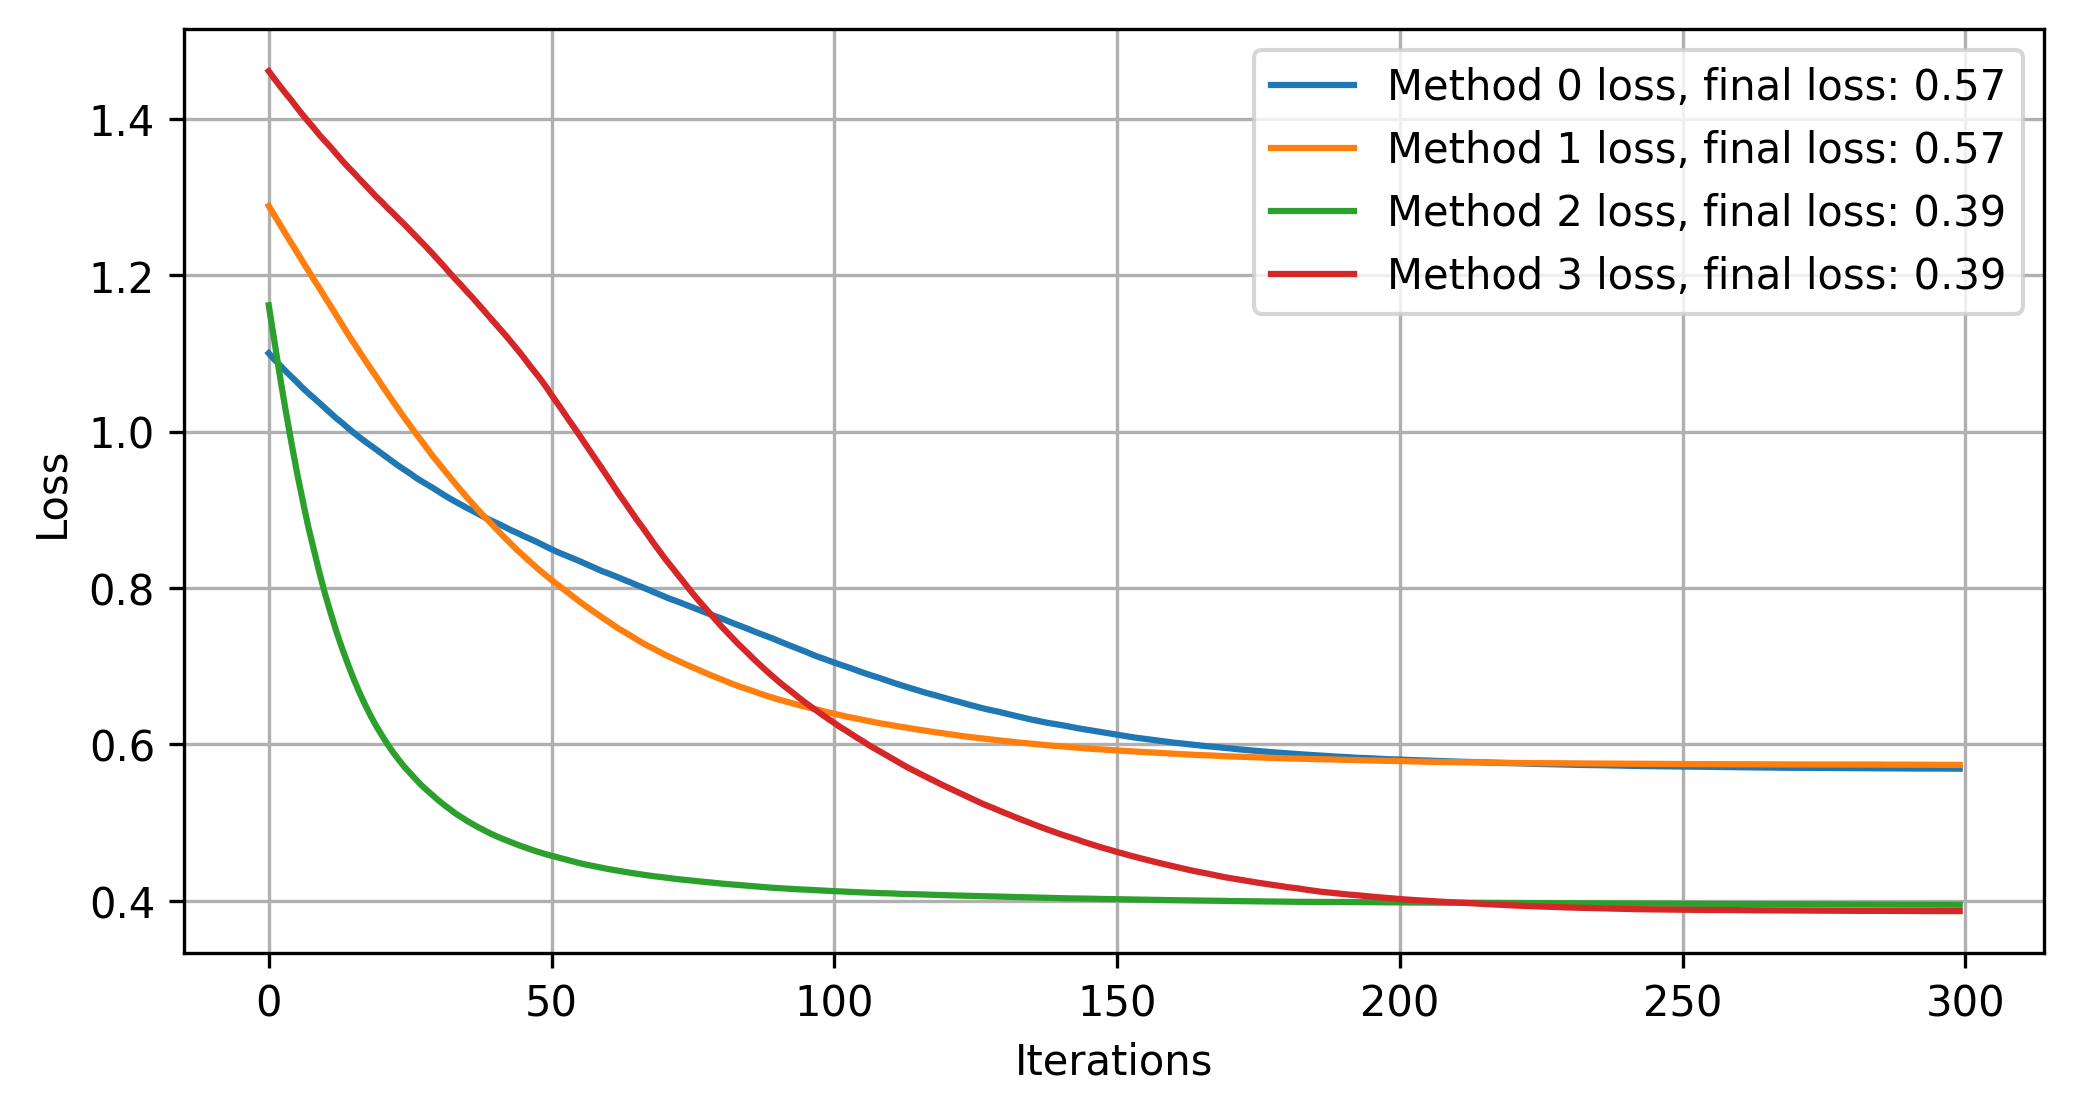
\includegraphics[width=\textwidth]{Artefact/Appendices/loss.png}
        \centerline{a) Loss funtion values of four classifiers in 300 steps}
    \end{subfigure}
    \begin{subfigure}{\textwidth}
        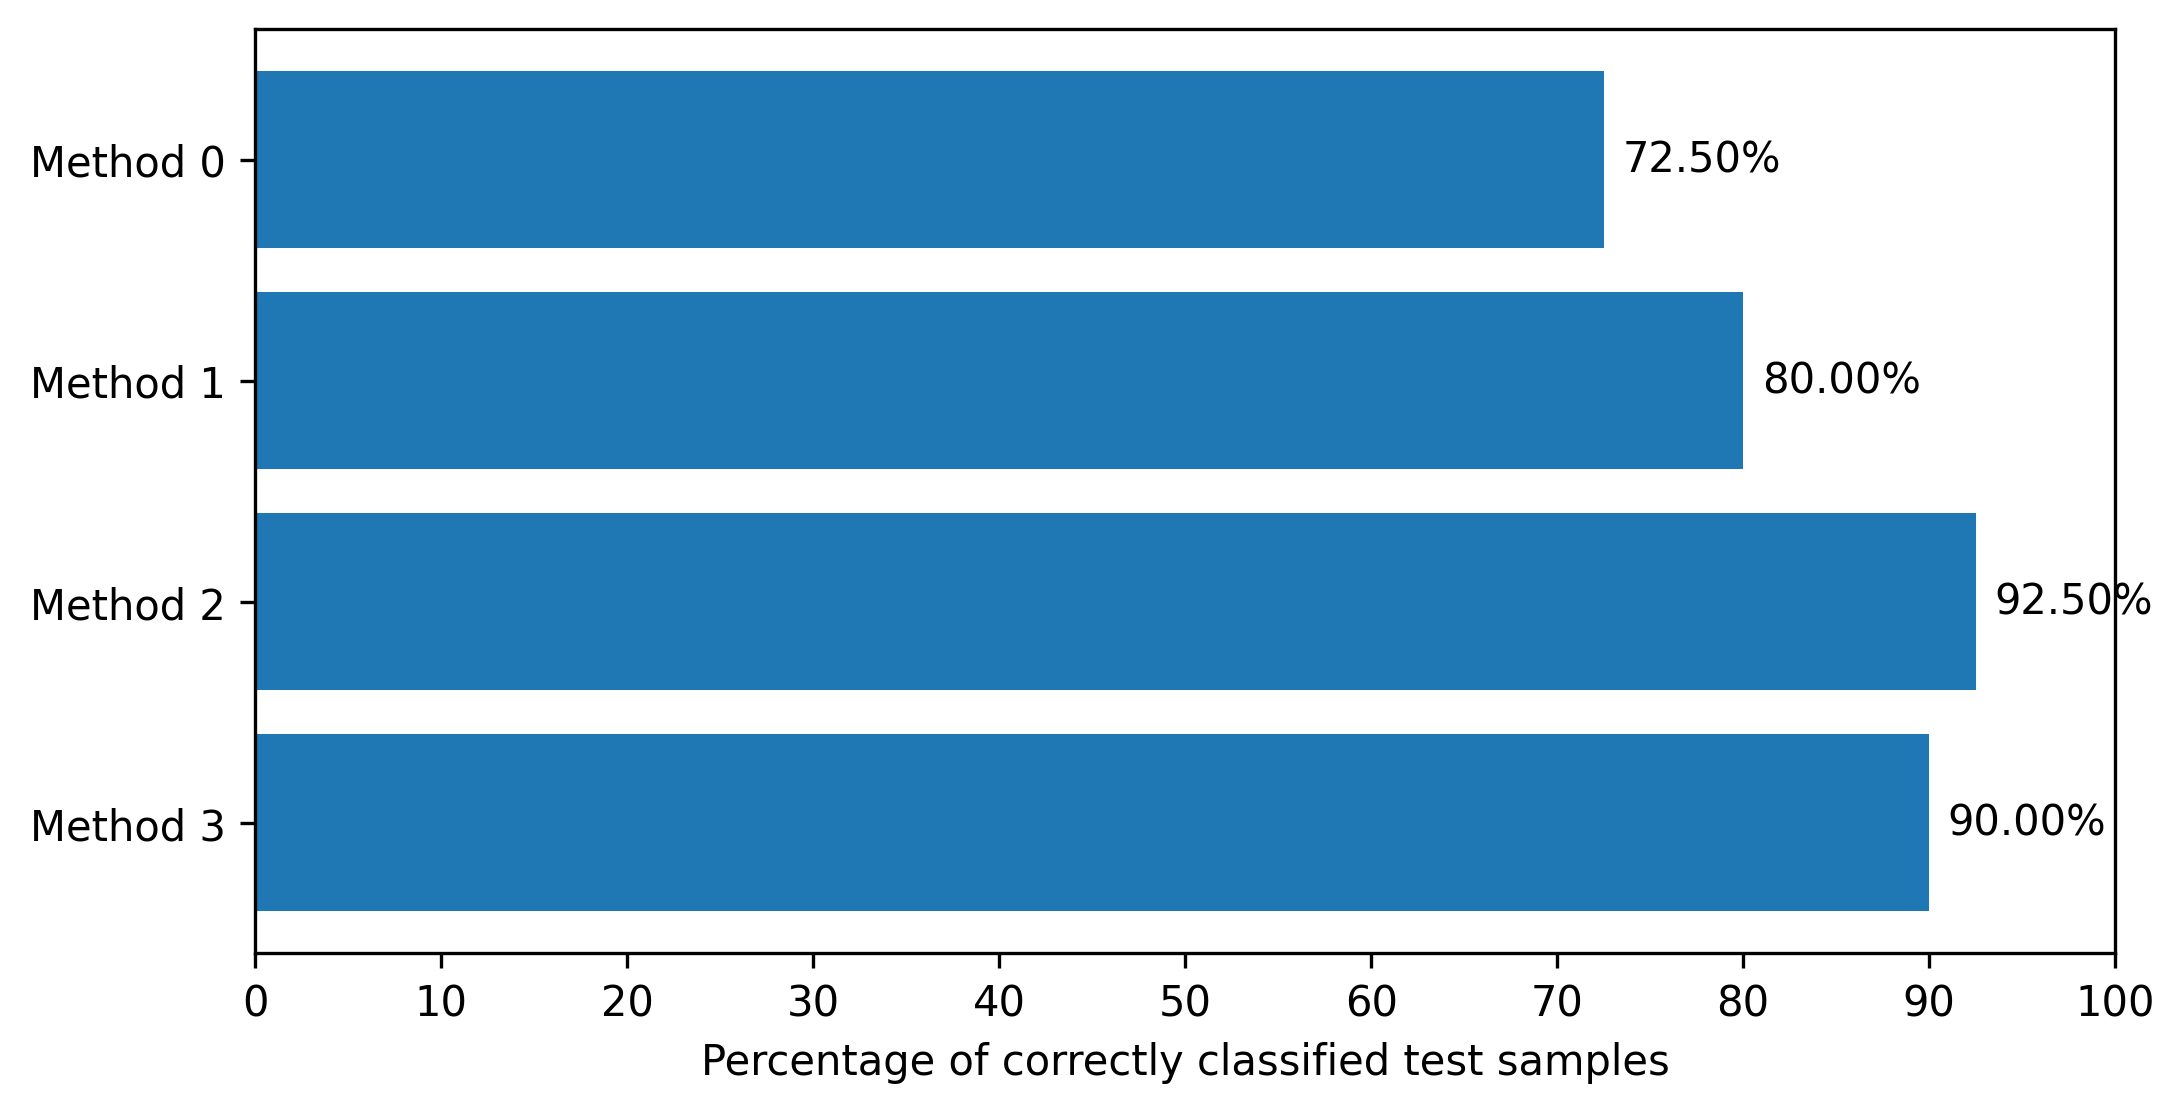
\includegraphics[width=\textwidth]{Artefact/Appendices/accuracy.png}
        \centerline{b) Accuracy score of four classifiers}
    \end{subfigure}

    \caption{
        Comparison of the loss values per iteration of gradient descent for the ansatzes with four treatments applies.
        We measure the accuracy of prediction with a set of 20 testing datapoint.
    }
    \label{Fig: Plot Loss and Accuracy}
\end{figure}
